\documentclass{beamer}
\usepackage{amsmath}
\usepackage{amssymb}
\usepackage{tikz}
\usepackage{booktabs}

% Theme
\usetheme{Madrid}
\usecolortheme{default}

% Title page info
\title{Finding Book Friends with Clustering}
\subtitle{Machine Learning Approach to Reader Compatibility}
\author{Hardcover Book Friend Finder}
\date{\today}

\begin{document}

% ============================================================================
% SLIDE 1: Results Comparison
% ============================================================================

\begin{frame}{Why Not Just Recommend Popular Books?}

\textbf{We tested collaborative filtering vs. popularity baseline:}

\vspace{0.5cm}

\begin{table}
\centering
\begin{tabular}{lc}
\toprule
\textbf{Method} & \textbf{Precision@10} \\
\midrule
Pure collaborative filtering & 2.16\% \\
Improved collaborative (filtered) & 2.45\% \\
\alert{Popularity baseline} & \alert{7.56\%} \\
Hybrid (50/50) & 8.83\% \\
\bottomrule
\end{tabular}
\end{table}

\vspace{0.5cm}

\textbf{Lesson:} Pure collaborative filtering performs \alert{worse} than just recommending popular books!

\textbf{Why?} 95.75\% sparsity - too much missing data

\textbf{Solution:} Hybrid approach works best (8.83\% vs 7.56\%)

\end{frame}

% ============================================================================
% SLIDE 2: Data Filtering and Computational Complexity
% ============================================================================

\begin{frame}{Data Filtering \& Scalability}

\begin{block}{Data Filtering}
Started with 1,000 Hardcover users and 45,203 books. Filtered to:
\begin{itemize}
    \item \textbf{Users with $\geq$ 20 ratings:} 246 users
    \item \textbf{Books with $\geq$ 5 users:} 2,547 books
    \item \textbf{Total possible:} $246 \times 2,547 = 626,562$ ratings
    \item \textbf{Actual interactions:} 26,598 (only 4.25\%)
\end{itemize}
\end{block}

\vspace{0.2cm}

\begin{block}{Computational Performance}
Training time and scalability (300 iterations, 20 features):
\begin{itemize}
    \item \textbf{Current dataset (246 users):} 8.1 seconds
    \item \textbf{Projected 10,000 users:} ~32.7 seconds
    \item \textbf{Projected 100,000 users:} ~5.2 minutes
    \item \textbf{Time per user:} ~33ms (scales linearly)
\end{itemize}
\end{block}

\end{frame}

% ============================================================================
% SLIDE 3: Masking Solution
% ============================================================================

\begin{frame}{The Masking Solution}

\begin{block}{Problem: 95.75\% Sparsity}
Most entries in the ratings matrix are \alert{unknown}, not negative ratings. We can't train on missing data!
\end{block}

\vspace{0.5cm}

\begin{block}{Solution: Masking Matrix $R$}
We use a \alert{mask matrix $R$} where:
\begin{equation*}
R[i,j] = \begin{cases}
1 & \text{if user } i \text{ interacted with book } j \\
0 & \text{otherwise (unread)}
\end{cases}
\end{equation*}

\vspace{0.3cm}

\textbf{Key insight:} Only train on known interactions (4.25\%), ignore unread books (95.75\%)

\vspace{0.3cm}

This prevents the model from trying to predict missing data and focuses learning on actual user preferences.
\end{block}

\end{frame}

% ============================================================================
% SLIDE 4: Matrix Factorization
% ============================================================================

\begin{frame}{Matrix Factorization: Learning User Preferences}

\begin{center}
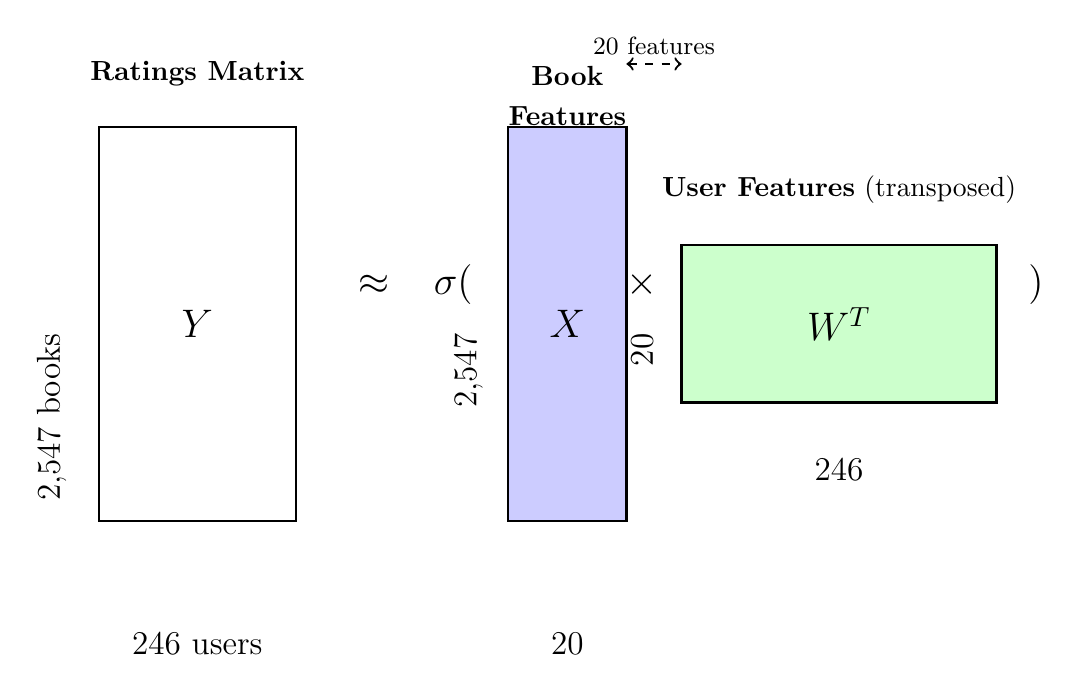
\begin{tikzpicture}[scale=1.0]
    % Y matrix (Ratings)
    \draw[thick] (0,0) rectangle (2.5,5);
    \node at (1.25,2.5) {\Large $Y$};
    \node[below] at (1.25,-1.3) {\large 246 users};
    \node[left,rotate=90] at (-0.6,2.5) {\large 2,547 books};
    \node[above] at (1.25,5.4) {\textbf{Ratings Matrix}};

    % Approximately equal
    \node at (3.5,3.0) {\Large $\approx$};

    % Sigmoid function
    \node at (4.5,3.0) {\Large $\sigma($};

    % X matrix (Book features)
    \draw[thick,fill=blue!20] (5.2,0) rectangle (6.7,5);
    \node at (5.95,2.5) {\Large $X$};
    \node[below] at (5.95,-1.3) {\large 20};
    \node[left,rotate=90] at (4.7,2.5) {\large 2,547};
    \node[above] at (5.95,5.4) {\textbf{Book}};
    \node[above] at (5.95,4.9) {\textbf{Features}};

    % Multiplication symbol
    \node at (6.9,3.0) {\Large $\times$};

    % W^T matrix (User features transposed)
    \draw[thick,fill=green!20] (7.4,1.5) rectangle (11.4,3.5);
    \node at (9.4,2.5) {\Large $W^T$};
    \node[below] at (9.4,0.9) {\large 246};
    \node[left,rotate=90] at (6.9,2.5) {\large 20};
    \node[above] at (9.4,3.9) {\textbf{User Features} (transposed)};

    % Closing parenthesis for sigmoid
    \node at (11.9,3.0) {\Large $)$};

    % Dimensions annotation
    \draw[<->,dashed,thick] (6.7,5.8) -- (7.4,5.8);
    \node[above] at (7.05,5.8) {\small 20 features};
\end{tikzpicture}
\end{center}

\vspace{0.3cm}

Each user gets a \alert{20-dimensional feature vector} describing their reading preferences

\end{frame}

% ============================================================================
% SLIDE 5: The Hybrid Method
% ============================================================================

\begin{frame}{The Hybrid Method: Best of Both Worlds}

\begin{block}{Why Hybrid?}
Pure collaborative filtering (2.16\%) performed \alert{worse} than just recommending popular books (7.56\%)!
\end{block}

\vspace{0.3cm}

\begin{block}{The Solution: 50/50 Hybrid Approach}
Combine two recommendation strategies:

\vspace{0.3cm}

\begin{equation*}
\text{Final Score} = 0.5 \times \text{Popularity Score} + 0.5 \times \text{Collaborative Score}
\end{equation*}

\vspace{0.3cm}

\begin{itemize}
    \item \textbf{Popularity:} Recommend books many users liked (safe baseline)
    \item \textbf{Collaborative:} Recommend based on user's learned preferences (personalization)
\end{itemize}
\end{block}

\vspace{0.3cm}

\begin{block}{Result}
\textbf{8.83\% precision} - outperforms both individual methods! (17\% better than popularity alone)
\end{block}

\end{frame}

% ============================================================================
% SLIDE 6: Clustering for Friend Finding
% ============================================================================

\begin{frame}{Clustering: Finding Your Reading Tribe}

\textbf{Goal:} Group users with similar reading preferences

\vspace{0.5cm}

\begin{block}{How It Works}
\begin{enumerate}
    \item Start with each user's 20-dimensional feature vector
    \item \textbf{Normalize} the vectors (make them unit length)
    \item Use \alert{K-means clustering} to group similar users
    \item Tested different cluster counts, found \alert{K=13} is optimal
\end{enumerate}
\end{block}

\vspace{0.3cm}

\begin{block}{Finding Friends within Your Cluster}
\begin{itemize}
    \item Calculate \textbf{dot product} (cosine similarity) with each cluster member
    \item Higher similarity = better friend match
    \item Show shared books as conversation starters
\end{itemize}
\end{block}

\vspace{0.3cm}

\textbf{Result:} 13 distinct reading groups (Fantasy Fans, Sci-Fi Enthusiasts, etc.)

\end{frame}

\end{document}
